% !TEX root = MATLAB_OOP_Blair.tex

% ============================================================
% ============================================================
% ============================================================
\section{Built-in Classes}
% ============================================================
% ============================================================
% ============================================================

We will gain some experience with classes with MATLAB's built-in classes. A class defines a composite data type. When we define \texttt{n = 71.9}, we say that \texttt{n} is a variable of type \texttt{double}. Similarly, a variable belonging to some class is called an \textbf{object}. You'll also hear it said that we \textit{instantiate} an object of a certain class, or that some object is an instance of some class.  If we were to write an analogy, we might write \texttt{type:variable::class:object}. We can say that a class is a generalization of the concept of a variable.

Like a \texttt{struct}, an object may have multiple elementary data types embedded in it. In a \texttt{struct}, the constituent data elements are called ``fields,'' but in an object the constituent data elements are called ``properties.''

% ============================================================
% ============================================================
\subsection{The \texttt{datetime} Class}
% ============================================================
% ============================================================
The \texttt{datetime} class is provided to allow users to create and manipulate dates.

% ============================================================
\subsubsection{Creating a New \texttt{datetime} Object}
% ============================================================

We can instantiate a \texttt{datetime} object, \texttt{x}, as follows:
% vvv------------------------------------------------------------vvv
\begin{lstlisting}[style=Matlab-editor, caption={This input to the MATLAB Command Window input uses the \texttt{datetime()} constructor method to instantiate a \texttt{datetime} object, \texttt{x}.}]
>> x = datetime('now')

x = 

  datetime

   17-Apr-2021 19:44:34

>> class(x)

ans =

    'datetime'
\end{lstlisting}
% ^^^------------------------------------------------------------^^^
MATLAB automatically reports that this is a \texttt{datetime} object, and the \texttt{class} function is in agreement with this.

% ============================================================
\subsubsection{Properties}
% ============================================================
Building on the previous code block, we can then use the \texttt{properties()} function to discover what properties the object \texttt{x} has. Then, we can reference those properties using the dot syntax:
% vvv------------------------------------------------------------vvv
\begin{lstlisting}[style=Matlab-editor, caption={The \texttt{properties()} function lists the accessible properties of the \texttt{x} object.}]
>> properties(x)

Properties for class datetime:

    Format
    TimeZone
    Year
    Month
    Day
    Hour
    Minute
    Second
    
>> x.Year

ans =

        2021

>> disp(['Month: ', num2str(x.Month)])
Month: 4
\end{lstlisting}
% ^^^------------------------------------------------------------^^^


% ============================================================
\subsubsection{Method Functions}
% ============================================================

Any function associated with a class is called a \textbf{method function}, or simply a ``method.'' Methods define how objects can be used and manipulated, and how data contained in functions can be accessed.

The \texttt{datetime} function is actually a special method called a \textbf{constructor method}. This defines how a new object is instantiated for the class. In the previous code block, we use the string \texttt{'now'} as an input to the constructor \texttt{datetime}. This caused \texttt{datetime} to obtain the current computer clock time and form a \texttt{datetime} object. The \texttt{datetime} constructor may also be used to create a \texttt{datetime} object for a specific day:
% vvv------------------------------------------------------------vvv
\begin{lstlisting}[style=Matlab-editor, caption={A \texttt{datetime} object is created to represent October 5, 2016 as a birthday.}]
>> bday = datetime(2016, 10, 5)

bday = 

  datetime

   05-Oct-2016

>> age = between(bday, datetime('now'))

age = 

  calendarDuration

   4y 6mo 13d 0h 24m 30.366s

\end{lstlisting}
% ^^^------------------------------------------------------------^^^
 You can use \texttt{help datetime} to discover other ways to use the \texttt{datetime} constructor.

Other methods can be defined to access, display or manipulate the data in an object. For example, \texttt{between} is a \texttt{datetime} function designed to find the duration between two \texttt{datetime} objects, as in lines 9-15 of the above listing.



% ============================================================
% ============================================================
\subsection{MATLAB Graphics Classes}
% ============================================================
% ============================================================

If you've used MATLAB graphics, you've already used classes and objects, whether you realize it or not. MATLAB graphics make heavy use of object-oriented programming.

% ============================================================
\subsubsection{The \texttt{Figure} Class}
% ============================================================

Consider the following Command Window session, which creates a new figure:
% vvv------------------------------------------------------------vvv
\begin{lstlisting}[style=Matlab-editor, caption={A new figure is created in the MATLAB Command Window.}]
>> myFig = figure

myFig = 

  Figure (1) with properties:

      Number: 1
        Name: ''
       Color: [0.9400 0.9400 0.9400]
    Position: [617 599 560 420]
       Units: 'pixels'

  Show all properties
  
>> ishandle(myFig)

ans =

  logical

   1
>> m = 7; ishandle(m)

ans =

  logical

   0
>> myFig.Position

ans =

   617   597   560   420

>>
\end{lstlisting}
% ^^^------------------------------------------------------------^^^
This creates the blank figure depicted in Fig.\ \ref{fig:NewBlankFig}. The Command Window output reports that the variable \texttt{myFig} actually is an object of class \texttt{Figure}. It also lists some of the most important properties of \texttt{myFig}, and you could see more properties by clicking on \texttt{all prooperties} in the Command Window.

The variable \texttt{myFig} is a special kind of variable called a \textbf{handle}. A handle is a variable that allows us to reference a MATLAB graphics object (objects of class \texttt{Figure}, \texttt{Axes}, \texttt{Line}, etc.), and line 15 demonstrates the use of \texttt{ishandle()} to verify \texttt{myFig} as a handle. Line 22 also demonstrates what happens when the argument to \texttt{ishandle} is a non-handle variable. Handles are useful if we wish to manipulate graphics objects using MATLAB code.  Line 29 demonstrates how we might obtain the properties of \texttt{myFig} for future use. Here, we have obtained the \((x,y)\)-coordinate of the lower-left corner of the figure, as well as its width and height, with all units in pixels. We also could adjust the figure position by reassigning these values using dot syntax, with a command like  \texttt{myFig.Position = [x y w h]} for some previously-defined \texttt{x}, \texttt{y}, \texttt{w}, and \texttt{h}. 

% vvv------------------------------------------------------------vvv
\begin{figure}[htbp] %  figure placement: here, top, bottom, or page
   \centering
   \subfigure[ \label{fig:NewBlankFig}]{\includegraphics[height=2.5in]{graphics/NewFig1.png}\label{fig:NewBlankFig}}
   \quad
   \subfigure[ \label{fig:NewBlankAx}]{\includegraphics[height=2.5in]{graphics/Fig01_with_axes.png}\label{fig:NewAxesFig}}
   \caption{(a) A new, blank figure. (b) A new, blank axes is added to the figure.}
   \label{fig:NewFigNewAx}
\end{figure}
% ^^^------------------------------------------------------------^^^

A subsequent use of a command like \texttt{newerFig = figure} command will create a new figure with number 2, and this figure may be referenced using the handle \texttt{newerFig}. When the \texttt{figure()} command is invoked with a handle to an existing figure, such as \texttt{figure(someHandle)}, the figure referenced by \texttt{someHandle} is brought to the top, shown in front of all other MATLAB figures, and it is designated as the \textbf{current figure}. Subsequent plotting commands will occur in the current figure. The current figure also may be referenced by the command \texttt{gcf}, which is short for ``get current figure.''
% ============================================================
\subsubsection{The \texttt{Axes} Class}
% ============================================================

If we continue the Command Window session from the previous listing, we can add a blank axes to the pre-existing figure as follows:
% vvv------------------------------------------------------------vvv
\begin{lstlisting}[style=Matlab-editor, caption={A new, blank axes is added to the figure.}]
>> myAx = axes

myAx = 

  Axes with properties:

             XLim: [0 1]
             YLim: [0 1]
           XScale: 'linear'
           YScale: 'linear'
    GridLineStyle: '-'
         Position: [0.1300 0.1100 0.7750 0.8150]
            Units: 'normalized'

  Show all properties

>> 
\end{lstlisting}
% ^^^------------------------------------------------------------^^^
Note that if \texttt{myAx} is embedded in \texttt{myFig},  an entry for this axes is made in the \texttt{myFig.Children} property:
% vvv------------------------------------------------------------vvv
\begin{lstlisting}[style=Matlab-editor, caption={When \texttt{myAx} is embedded in \texttt{myFig}, the \texttt{myFig.Children} property also may be used to reference the new axes object.}]
>> myFig.Children  % this points to an Axes object

ans = 

  Axes with properties:

             XLim: [0 1]
             YLim: [0 1]
           XScale: 'linear'
           YScale: 'linear'
    GridLineStyle: '-'
         Position: [0.1300 0.1100 0.7750 0.8150]
            Units: 'normalized'

  Show all properties

>>
\end{lstlisting}
% ^^^------------------------------------------------------------^^^
The new axes also may be referenced using \texttt{myFig.Children}.

When multiple subplots are defined within the current figure, the \texttt{Children} property of the current axes is an array:
% vvv------------------------------------------------------------vvv
\begin{lstlisting}[style=Matlab-editor, caption={Multiple \texttt{Axes} objects are added to \texttt{myFig}. \texttt{MyFig.Children} is an array, and each subplot now may be referenced as an element of \texttt{MyFig.Children} or by any handle associated with that subplot.}]
>> plot_a = subplot(2,1,1) % create an upper subplot

plot_a = 

  Axes with properties:

             XLim: [0 1]
             YLim: [0 1]
           XScale: 'linear'
           YScale: 'linear'
    GridLineStyle: '-'
         Position: [0.1300 0.5838 0.7750 0.3412]
            Units: 'normalized'

  Show all properties

>> plot_b = subplot(2,1,2) % create a lower subplot

plot_b = 

  Axes with properties:

             XLim: [0 1]
             YLim: [0 1]
           XScale: 'linear'
           YScale: 'linear'
    GridLineStyle: '-'
         Position: [0.1300 0.1100 0.7750 0.3412]
            Units: 'normalized'

  Show all properties

>> myFig.Children % now the figure has a two child Axes objects

ans = 

  2x1 Axes array:

  Axes
  Axes

>> myFig.Children(1) % points to the first Axes in the array

ans = 

  Axes with properties:

             XLim: [0 1]
             YLim: [0 1]
           XScale: 'linear'
           YScale: 'linear'
    GridLineStyle: '-'
         Position: [0.1300 0.1100 0.7750 0.3412]
            Units: 'normalized'

  Show all properties

>> myFig.Children(2) % points to the second Axes in the array

ans = 

  Axes with properties:

             XLim: [0 1]
             YLim: [0 1]
           XScale: 'linear'
           YScale: 'linear'
    GridLineStyle: '-'
         Position: [0.1300 0.5838 0.7750 0.3412]
            Units: 'normalized'

  Show all properties

>> 
\end{lstlisting}
% ^^^------------------------------------------------------------^^^
 Here, the top subplot is referenced by both \texttt{MyFig.Children(1)} and \texttt{plot\_a}; and, \texttt{MyFig.Children(2)} and \texttt{plot\_b} both are handles for the bottom subplot.
 
 
 % ============================================================
\subsubsection{The \texttt{Line} Class}
% ============================================================

When we plot data, we make \texttt{Line} objects. The following command plots two lines in one axes:
% vvv------------------------------------------------------------vvv
\begin{lstlisting}[style=Matlab-editor, caption={Two data sets are plotted on one \texttt{Axes} object.}]
>> x = linspace(-1, 1, 201);
% Plot two lines, with data_plot as a reference to the lines
data_plot = plot(x, sin(2*pi*x), x, cos(2*pi*x), 'LineWidth', 2)

data_plot = 

  2x1 Line array:

  Line
  Line

>> thisAx = gca; thisFig = gcf; thisAx

thisAx = 

  Axes with properties:

             XLim: [-1 1]
             YLim: [-1 1]
           XScale: 'linear'
           YScale: 'linear'
    GridLineStyle: '-'
         Position: [0.1300 0.1100 0.7750 0.8150]
            Units: 'normalized'

  Show all properties

>> thisAx.Children % the children of thisAx are Line objects

ans = 

  2x1 Line array:

  Line
  Line

>> 
\end{lstlisting}
% ^^^------------------------------------------------------------^^^
This code produced the \texttt{Figure}, \texttt{Axes}, and plot of Figure \ref{fig:MultiLinePlot}. The result is two line objects, which may be referenced in two ways: (1) using the elements of the \texttt{data\_plot} array [lines 5-10]; and (2) as children of the \texttt{Axes} object [lines 29-36]. Additionally, we obtain handles (line 28) to the current axes (\texttt{thisAx}) and current figure (\texttt{thisFig}) using \texttt{gca} (short for \textit{get current axes}) and \texttt{gcf} (short for \textit{get current figure}).

Then, we may also reference the two lines using \texttt{thisAx.Children}. Recall that the \texttt{Axes} object is a child object to the \texttt{Figure} object, contained in the \texttt{Figure} property \texttt{Children}. The \texttt{Line} objects, however, are listed as children in the \texttt{Children} property of the \texttt{Axes} object \texttt{thisAx}.

% vvv------------------------------------------------------------vvv
\begin{figure}[htbp] %  figure placement: here, top, bottom, or page
   \centering
   \subfigure[Initial plot.\label{fig:TwoLines}]{\includegraphics[height=2.6in]{graphics/FigTwoLines.png}}
   \quad
   \subfigure[After setting \texttt{data\_plot(1).LineStyle = \'--\'}. \label{fig:TwoLines_dashed}]{\includegraphics[height=2.6in]{graphics/FigTwoLines_dashed.png}}   
   \caption{Two data sets are plotted in one \texttt{Axes} object.}
   \label{fig:MultiLinePlot}
\end{figure}
% ^^^------------------------------------------------------------^^^

Let us inspect the properties of the \texttt{Line} object referenced by \texttt{data\_plot(1)}:
% vvv------------------------------------------------------------vvv
\begin{lstlisting}[style=Matlab-editor, caption={The properties of \texttt{data\_plot(1)}.}]
>> data_plot(1) % get properties of

ans = 

  Line with properties:

              Color: [0 0.4470 0.7410]
          LineStyle: '-'
          LineWidth: 2
             Marker: 'none'
         MarkerSize: 6
    MarkerFaceColor: 'none'
              XData: [1x201 double]
              YData: [1x201 double]
              ZData: [1x0 double]

  Show all properties

>> data_plot(1).LineStyle = '--';
\end{lstlisting}
% ^^^------------------------------------------------------------^^^
Line 19 shows how we can use the dot syntax to change the \texttt{LineStyle} property for \texttt{data\_plot(1)}, resulting in Figure \ref{fig:TwoLines_dashed}.

The \texttt{Line} object has special properties, \texttt{XData}, \texttt{YData}, and \texttt{ZData}. These contain the actual \(x\), \(y\), and \(z\) coordinates of data points plotted. Since there is no \texttt{ZData}, the plot is a 2D plot. If you wisxhed to change or animate your plot, it could be faster and visually smoother to simply update these properties, rather than replot the data with a new call to the \texttt{plot()} command. This will save time, since you do not have to clear the axes nor reformat it if you only adjust these special properties of the \texttt{Line} object.

An alternate and older way to get MATLAB graphics properties is to use the \texttt{get()} function. For example, \texttt{line\_col = get(data\_plot(1))} stores the red-green-blue (RBG) triple for \texttt{data\_plot(1)} in \texttt{line\_col}. This may also be done for any object of a MATLAB graphics class (\texttt{Figure}, \texttt{Axes}, \texttt{Line}, \texttt{Patch}, etc.).

Similarly, we may use the \texttt{set()} function to set properties of a MATLAB graphics object. While the dot syntax allows only one property to be modified at a time, the \texttt{set()} function allows multiple properties to be adjusted in one command. For example, we could use two commands to adjust the line style and line marker for \texttt{someLine}:
% vvv------------------------------------------------------------vvv
\begin{lstlisting}[style=Matlab-editor]
>> someLine.LineStyle = '--';
>> someLine.Marker = 'o';
\end{lstlisting}
% ^^^------------------------------------------------------------^^^
This may be done in one call of the \texttt{set()} function:
% vvv------------------------------------------------------------vvv
\begin{lstlisting}[style=Matlab-editor]
>> set(someLine, 'LineStyle', '--', 'Marker', 'o');
\end{lstlisting}
% ^^^------------------------------------------------------------^^^


% ============================================================
\subsubsection{The \texttt{Patch} Class}
% ============================================================

A MATLAB \texttt{Patch} object is a drawing of a closed polygon with straight edges. The polygon is specified by the the $x$-, $y$-, and (optional) $z$ coordinates of each vertex. The polygon is closed by connecting the last vertex to the first. Thus, it is redundant to have the first vertex and the last vertex as the same coordinate.

The basic syntax for the \texttt{patch()} function is \texttt{patch(X,Y,C)}. This creates a polygon of $N$ points, where \texttt{X} is a $1\times N$ vector of $x$ values, $Y$ is a $1\times N$ vector of $y$ values, and \texttt{C} is a color specifier. The color specifier can be a string to specify a basic color, such as \verb!'r'!, \verb!'g'!,\verb!'b'!,\verb!'c'!,\verb!'m'!,\verb!'y'!,\verb!'w'!, or \verb!'k'!; or, \texttt{C} may be a $3$-element RGB (red-blue-green) triple specifying an arbitrary color. For example: \verb!C = [1, 0, 0]! specifies elementary red; \verb!C = [0, 1, 0]! specifies green; \verb!C = [0, 0, 1]! specifies blue; \verb!C = [0, 0, 0]! specifies black; and \verb!C = [1, 1, 1]! specifies white.

As an example, I provide the listing of a \texttt{basicPatch.m} script. The patch is defined in lines 3-7, and following lines of code provide formatting.
% vvv------------------------------------------------------------vvv
\begin{lstlisting}[style=Matlab-editor,label=basicPatch,caption={Listing of the script \texttt{basicPatch.m}.}]
% basicPatch.m

x = [-1 -1 1 1]; % specify x-values for vertices
y = [-1 1 1 -1]; % specify y-values for vertices
C = [0.75 0 0.75]; % specify a purple-ish color

newSquare = patch(x, y, C)
set(gca, 'FontName', 'Times', 'FontSize', 20); % format the current axes
grid on;

xlim([-3 3]); % adjust the x-limits of the axis
ylim([-3 3]); % adjust the y-limits of the axis

xlabel('$x$ (m)', 'Interpreter', 'latex') % add an x-label
ylabel('$y$ (m)', 'Interpreter', 'latex') % add a y-label
\end{lstlisting}
% ^^^------------------------------------------------------------^^^
The output of the \texttt{basicPatch.m} script is shown in Fig.\ \ref{fig:basicPatchOutput}.

% vvv------------------------------------------------------------vvv
\begin{figure}[htbp] %  figure placement: here, top, bottom, or page
   \centering
   \subfigure[ ]{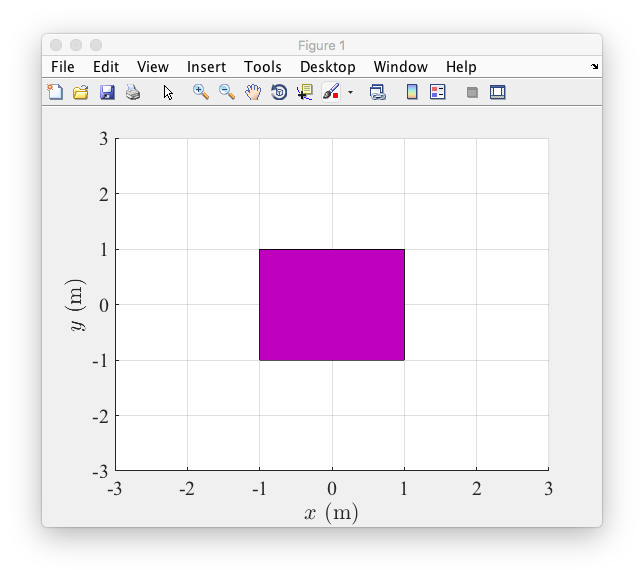
\includegraphics[width=0.475\textwidth]{graphics/basicPatchOutGraphical.png} \label{subfig:basicPatchOutputGraph}}
   \subfigure[ ]{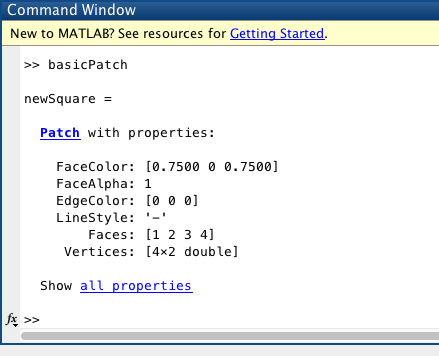
\includegraphics[width=0.475\textwidth]{graphics/basicPatchOutText.png} \label{subfig:basicPatchOutputText}}
   \caption{Graphical and Command Window output of the \texttt{basicPatch.m} script of Listing \ref{basicPatch}.}
   \label{fig:basicPatchOutput}
\end{figure}
% ^^^------------------------------------------------------------^^^

%The unsupressed output of Line 7 lists some properties of the \texttt{patch} object.
The \texttt{Patch} object is centered at the origin in Fig.\ \ref{subfig:basicPatchOutputGraph}. An example of a simple modification to this is to translate the patch by the vector $(\Delta x, \Delta y)$. To do this, we define $\Delta x$ and $\Delta y$, and add these to the original \texttt{XData} and \texttt{YData} properties of the \texttt{newSquare} object. This can be done in the Command Window using the \texttt{set()} function:
% vvv------------------------------------------------------------vvv
\begin{lstlisting}[style=Matlab-editor,label=basicPatchDisplace,caption={A Command Window modification to the \texttt{patch} defined in Listing \ref{basicPatch}. Line 1 is used to specify the $x$- and $y$-components of the displacement. The displacement is then applied to the original \texttt{XData} and \texttt{YData} properties, and the result of the addition is the value component of a property-value pair in the \texttt{set()} function.}]
>> Dx = -2; Dy = 1.5;
>> set(newSquare, 'XData', newSquare.XData + Dx, 'YData', newSquare.YData + DY)
\end{lstlisting}
% ^^^------------------------------------------------------------^^^
The syntax here is \verb!set(obj, Prop1, Val1, Prop2, Val2, ...)!, where \texttt{obj} is the object we wish to modify, and we use property-value pairs to assign new object properties. The displaced \texttt{patch} object is displayed in Fig.\ \ref{fig:basicPatchDisplaced}. Similar modifications may be made to a \texttt{line}-class object.

% vvv------------------------------------------------------------vvv
\begin{figure}[htbp] %  figure placement: here, top, bottom, or page
   \centering
   \subfigure[ \label{fig:basicPatchDisplaced}]{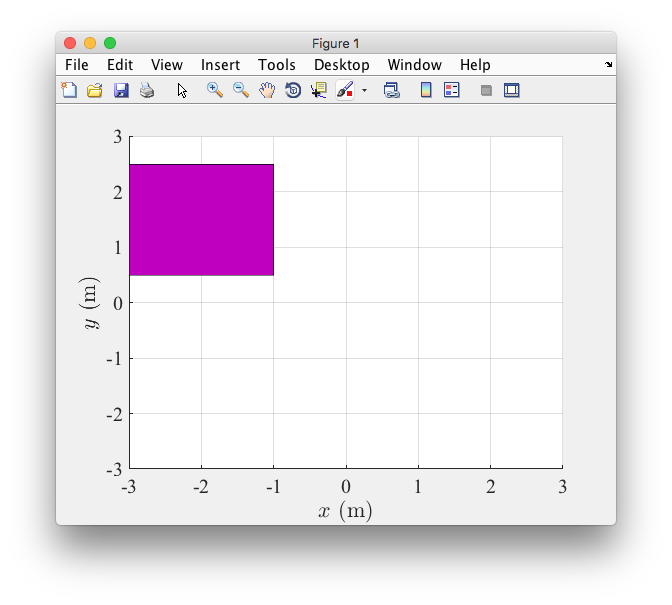
\includegraphics[width=0.475\textwidth]{graphics/basicPatchDisplaced.png}}
   \subfigure[ \label{fig:AxisEq}]{\includegraphics[width=0.475\textwidth]{graphics/FigPatchAxisEqual.png} \label{subfig:basicPatchOutputGraph}}
      \caption{The \texttt{patch} object created using \texttt{basicPatch.m} is modified by using the \texttt{set()} function using the code of Listing \ref{basicPatchDisplace}. The resulting \texttt{patch} no longer sits at the origin.}

\end{figure}
% ^^^------------------------------------------------------------^^^

You may have noticed that the aspect ratio is not equal for the plot of Figure \ref{fig:basicPatchDisplaced}. This may be improved using the \texttt{axis()} function:
% vvv------------------------------------------------------------vvv
\begin{lstlisting}[style=Matlab-editor,label=basicPatchDisplace,caption={A Command Window modification to the \texttt{patch} defined in Listing \ref{basicPatch}. Line 1 is used to specify the $x$- and $y$-components of the displacement. The displacement is then applied to the original \texttt{XData} and \texttt{YData} properties, and the result of the addition is the value component of a property-value pair in the \texttt{set()} function.}]
>> axis(gca, 'equal')
\end{lstlisting}
% ^^^------------------------------------------------------------^^^
This may adjust the \(x\)-limits and \(y\)-limits of the plot or only the positioning of the \texttt{Axis} object to get an equal aspect ratio.


For more information about the \texttt{patch} class, type \texttt{doc patch} in the MATLAB Command Window, or do an Internet search.


% ============================================================
\subsubsection{Animations using MATLAB Handle Graphics}
% ============================================================

When making animations in MATLAB, we may (1) replot each frame, or we may simply (2) adjust \texttt{XData}, \texttt{YData}, and \texttt{ZData} for objects in the plot for each frame. Method 2 is to be preferred, especially for interactive animations, because it is faster and avoids reconstructing and reformatting the plot. This results in a smoother experience for the user. It also may be helpful to set the axes limits using \texttt{xlim} and \texttt{ylim} so that relative positions of graphical objects is readily apparent between frames and the graphics for each frame all are plotted against the same background.

For an animation example and tutorial, see this demonstration on \myhref{https://youtu.be/mOwX0mfjJtQ}{animating ``rain drops''} in MATLAB.

